%!TEX root = ../report.tex
%*******************************************************************************
%                              Implementation                                  %
%*******************************************************************************


\chapter{Implementation}


%******************************** Section 5.1 *********************************%
\section{Introduction}
    After fixing the system design and choosing the appropriate hardware, it is time to implement the worker.
    The implementation consists of two parts, assembling the hardware components and preparing the software.
    To test the worker we developed Dpps for ARM architecture and integrated them in the iExec platform.
    In the last section we illustrate the work that has been done with some pictures of the worker prototype.

%******************************** Section 5.2 *********************************%
\section{Work environment}

   \begin{itemize}
        \item \textit{Amazon AWS instance: }
        The scheduler is running on this machine, it is packaged as a docker image and uses a mysql
        database. Also an Ethereum blockchain client (Geth) is installed on the EC2 instance so the scheduler
        and the worker will be using this node.

        \item \textit{A cluster of 3 Raspberry Pi boards: }
        First, what is Raspberry Pi ? The Raspberry Pi is a low cost, credit-card sized computer that plugs
        into a computer monitor or TV, and uses a standard keyboard and mouse. It is a capable little device
        that enables people of all ages to explore computing, and to learn how to program in languages like
        Scratch and Python. It is capable of doing everything we  expect a desktop computer to do, from
        browsing the internet and playing high-definition videos, to making spreadsheets, word-processing, and
        playing games\cite{raspberry-pi}.

        The worker software is installed on the board, all the binary files are packaged in a docker image
        and pushed to docker hub. The worker downloads the required version of the image and runs it.

        \item \textit{The client machine: }
        We use a client machine to test the infrastructure. We use the iExec SDK to deploy Dapps with ARM
        binaries, then we add available orders in the database and buy them. Those orders are executed on
        the Raspberry Pi workers.
   \end{itemize}

%******************************** Section 5.3 *********************************%
\section{Development technologies}
    We used different technologies for each phase of the project.

   \begin{itemize}
        \item \textit{Development}
            \begin{itemize}
                \item \textit{Java: }
                Java is a general-purpose computer-programming language that is concurrent, class-based,
                object-oriented, and specifically designed to have as few implementation dependencies as possible.
                It is intended to let application developers "write once, run anywhere" (WORA), meaning that compiled
                Java code can run on all platforms that support Java without the need for recompilation. Java
                applications are typically compiled to bytecode that can run on any Java virtual machine (JVM)
                regardless of computer architecture. It is the language used by the XtremWeb middleware.
                \item \textit{Python: }
                Python is an interpreted high-level programming language for general-purpose programming. Created by
                Guido van Rossum\cite{guido-van-rossum} and first released in 1991, Python has a design philosophy that emphasizes code
                readability, notably using significant whitespace. It provides constructs that enable clear programming
                on both small and large scales.
                \item \textit{Opencv: }
                OpenCV (Open Source Computer Vision Library) is an open source computer vision and machine learning
                software library. OpenCV was built to provide a common infrastructure for computer vision applications
                and to accelerate the use of machine perception in the commercial products. Being a BSD-licensed product,
                OpenCV makes it easy for businesses to utilize and modify the code.
                \item \textit{Git: }
                Git is a version control system for tracking changes in computer files and coordinating work on those
                files among multiple people. It is primarily used for source code management in software development,
                but it can be used to keep track of changes in any set of files. As a distributed revision control system,
                it is aimed at speed, data integrity, and support for distributed, non-linear workflows. Git was created
                by Linus Torvalds in 2005 for development of the Linux kernel, with other kernel developers contributing
                to its initial development. Its current maintainer since 2005 is Junio Hamano.
            \end{itemize}

        \item \textit{Configuration management}
            \begin{itemize}
                \item \textit{Ansible: }
                Ansible is open source software that automates software provisioning, configuration management, and
                application deployment. Ansible connects via SSH, remote PowerShell or via other remote APIs.
                We used it to install dependencies (docker, npm...) on the workers cluster.
            \end{itemize}

        \item \textit{Deployment}
            \begin{itemize}
                \item \textit{Docker: }
                Docker is a computer program that performs operating-system-level virtualization,
                also known as "containerization". It was first released in 2013 and is developed by
                Docker, Inc. Docker is used to run software packages called "containers". In a typical
                example use case, one container runs a web server and web application, while a second
                container runs a database server that is used by the web application. Containers are
                isolated from each other and bundle their own tools, libraries and configuration files;
                they can communicate with each other through well-defined channels. All containers are
                run by a single operating system kernel and are thus more lightweight than virtual
                machines. Containers are created from "images" that specify their precise contents.
                Images are often created by combining and modifying standard images downloaded from
                repositories.
                \item \textit{Docker Swarm: }
                Docker Swarm is a clustering and scheduling tool for Docker containers. With Swarm, IT
                administrators and developers can establish and manage a cluster of Docker nodes as a single
                virtual system. Swarm mode also exists natively for Docker Engine, the layer between the OS
                and container images. Swarm mode integrates the orchestration capabilities of Docker Swarm
                into Docker Engine 1.12 and newer releases.
                \item \textit{Geth: }
                Geth is an implementation of an Ethereum node in the Go programming language. In simpler terms,
                Geth is a program which serves as a node for the Ethereum blockchain, and via which a user can
                mine Ether and create software which runs on the EVM – the Ethereum Virtual Machine.
                This software can be things like crypto tokens, decentralized apps, and more.
            \end{itemize}

        \item \textit{Testing}
            \begin{itemize}
                \item \textit{iExec SDK: }
                We used the SDK to deploy Dapps for ARM architecture on the platform. After getting the Dapp
                address we run tests to start tasks on the workers and get the result, which confirms that the
                worker is ready to accept jobs from any source.
            \end{itemize}

        \item \textit{Visualizing}
            \begin{itemize}
                \item \textit{Docker Swarm Visualizer: }
                A visualizer for Docker Swarm Mode using the Docker Remote API, Node.JS, and D3. It is a demo container
                that displays Docker services running on a Docker Swarm in a diagram. It displays also some basic
                informations of cluster's nodes.
                \item \textit{Weave Scope: }
                A monitoring, visualization and management tool for Docker \& Kubernetes. It automatically generates
                a map of application, enabling an intuitive understanding, monitoring, and controlling of containerized,
                microservices based application.
                \item \textit{Adminer: }            
                Adminer (formerly phpMinAdmin) is a full-featured database management tool written in PHP.
                Conversely to phpMyAdmin, it consist of a single file ready to deploy to the target server.
                Adminer is available for MySQL, PostgreSQL, SQLite, MS SQL, Oracle, Firebird, SimpleDB, Elasticsearch
                and MongoDB.
            \end{itemize}

    \end{itemize}

%******************************** Section 5.4 *********************************%
\section{Achievements}
    We fixed in previous chapters the functional and non-functional requirements of our project. We evaluate
    in this section the achieved work and to what point we satisfied those requirements.

    \subsection{Blockchain}
    The blockchain is a critical factor for the functioning of the worker. Although, it is its mission
    to ensure the creation of a wallet, we provide a tools to generate wallets for the cluster of workers
    using ansible and iExec SDK. This is necessary for the PoCo verification.

    \subsection{XtremWeb}
    In order to execute jobs sent by the scheduler without problems, we have to ensure that XtremWeb supports
    arm architecture. We altered the java code to add this feature.

    The XtremWeb software is packaged in a docker image, where all the dependencies are installed and the jar
    files are copied. The build of this image is being done on a build server in the cloud, so its architecture
    is x86. We used QEMU combined with Resin.io to cross-compile the ARM image on x86 machine.
    QEMU is a hosted virtual machine monitor: it emulates the machine's processor through dynamic binary
    translation and provides a set of different hardware and device models for the machine, enabling it to
    run a variety of guest operating systems. QEMU can also do emulation for user-level processes, allowing
    applications compiled for one architecture to run on another.

    Since the Raspberry pi board is limited in terms of performance, we tried to optimize the docker image to be
    as minimalistic as possible. There are many techniques to reduce the size of the image like multi-stage
    build and cache cleaning. We increased also the heap size for the java process in the case of
    Raspberry Pi worker.

    \subsection{Workers cluster}
    A computer cluster is a set of computers that work together so that they can be viewed as a single system.
    In our case we have a cluster of Raspberry Pi workers and it is so hard to control them independently.
    As a solution we use two key technologies.

    The first one is Ansible, which is a configuration management tool.
    Ansible gives the ability of checking the dependencies on the cluster machines, and checking the presence
    of wallets.

    The second revolutionary technology is Docker swarm which is a tool that allows to orchestrate a cluster
    of containers running instances of a (multiple) service(s). Swarm is mandatory to simplify this task
    because we can control all the cluster nodes from a single machine without having to connect to every node
    to check status or start processes. Starting and stopping the XtremWeb software have not been easier.

    \subsection{Positive energy}
    One of the big features of this project is the energy side. After multiple measurements and
    testing we got some interesting results. The worker can be almost autonomous and can run only with solar
    energy. With an average of 8 sun hours a day, the worker under stress can survive almost forever.

    \textbf{Statistics:}

    \textit{The battery performance:}

    \begin{itemize}
        \item Full battery + 1 Raspberry Pi worker under stress: The worker consumes a maximum of 1A per hour
        so it takes a duration of 48 hours to empty the battery.

        \item Full battery + 2 Raspberry Pi workers under stress: The two workers consume 1.7A as a maximum and
        can stay up and running for 24 hours.
    \end{itemize}

    \textit{The solar panel performance:}
    Under 8 sunny hours in a medium cloudy day, the panel charges the battery with enough electricity for 18
    hours while the worker is running simultaneously. This duration is not the required
    duration for a complete autonomy of the worker but in normal conditions the panel would provide enough
    charge for a continuous performance. We tested it for a duration of a week and the worker stayed up for
    all this period.

    \subsection{Usage of sensors to provide data}
    One of the missions of the worker is to simulate an IoT device, so we added to the worker the possibility
    to interact with the environment and get data from it. We used multiple types of sensors to get measures
    such as temperature, humidity, pressure (...) and send them to an external service. We used also a camera
    to monitor a room, the stream of data is analysed to detect motions which highlights here the concept
    of Edge Computing. The data is processed locally instead of sending it like it is to the cloud.

    \subsection{Development of Dapps to test the infrastructure}
    After preparing the worker, deploying all the environment (scheduler, blockchain node...) and testing
    the solar panel performance to get some statistics, it is time to test the worker with real tasks
    instead of just lunching the stress command. But before we can test it, we need Dapps that contains ARM
    binaries so they can be executed on the Raspberry Pi. This part took some important time and effort because
    we tried to develop some computation demanding applications. We opted in our choices for image processing
    and text to speech applications. We present in this subsection the developed Dapps and the results of the
    tests. Those Dapps are listed publicly on the iExec Dappstore so everyone can use them. Those dapps have
    the advantage of being Ethereum-ready so it is so simple for Ethereum developers to use them directly.

    \begin{itemize}
        \item \textit{Object detection: }
        It is a python Dapp that uses opencv to detect objects from images. It uses
        MobileNets\cite{mobile-nets} a Convolutional Neural Network for Mobile Vision Applications.
        We call these networks “MobileNets” because they are designed for resource constrained
        devices such as smartphones.
        The application takes a set of images as input, it passes them throw the
        Neural Network, it marks the objects and determines their positions in the images.
        Every output image contains the detected objects.

        \clearpage

        \begin{figure}[!h]\centering
            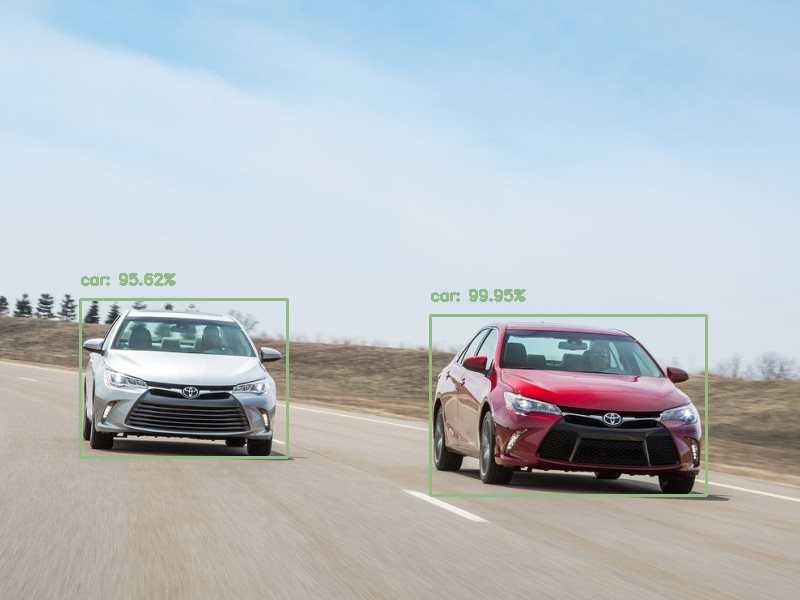
\includegraphics[width=.6\columnwidth]{6-Implementation/figs/object-detector-exp-1.jpg}
            \caption{Detected cars}
        \end{figure}

        \vspace{50px}

        \begin{figure}[!h]\centering
            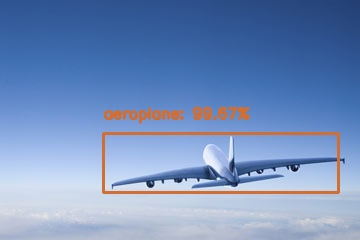
\includegraphics[width=.6\columnwidth]{6-Implementation/figs/object-detector-exp-2.jpg}
            \caption{Detected aeroplane object}
        \end{figure}

        Github repository\cite{object-detector}.

        \clearpage

        \item \textit{Image to text: }

        \begin{figure}[!h]\centering
            
\includegraphics[width=.3\columnwidth]{6-Implementation/figs/image-to-text-logo.png}
            \caption{Image to text Dapp logo}
        \end{figure}

        \vspace{50px}

        image2text is an Ethereum ready Dapp that applies google's tesseract-OCR engine to extract
        text from images. It is written in python and employs opencv and tesseract-ocr. The Dapp takes as
        input a set of images and returns, for each one of them, a file containing the extracted text.

        \vspace{50px}

        \begin{figure}[!h]\centering
            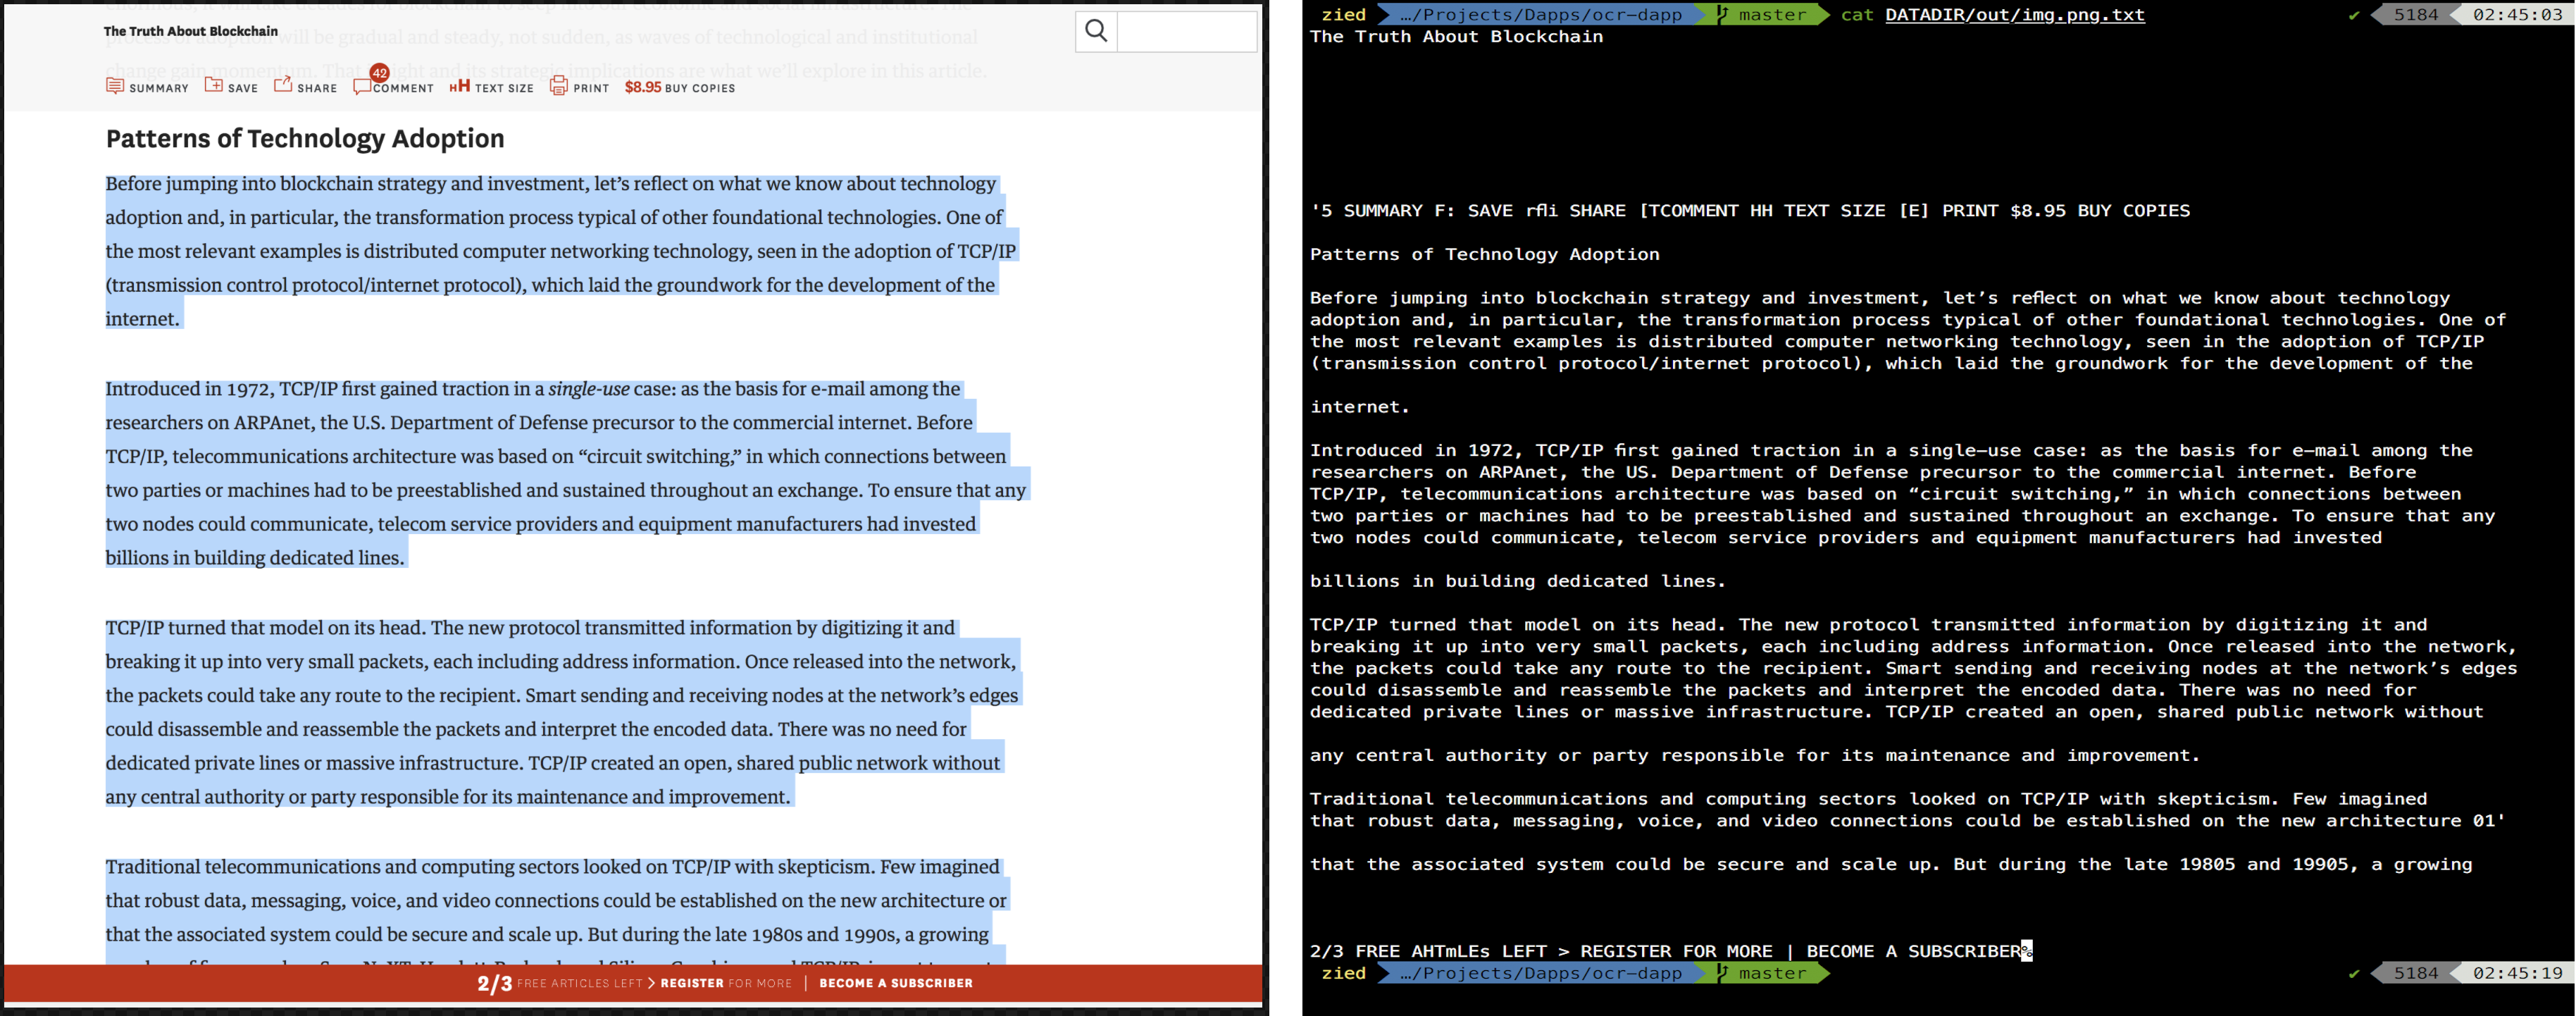
\includegraphics[width=\columnwidth]{6-Implementation/figs/image-to-text-exp.png}
            \caption{Extracted text from an image}
        \end{figure}

        Github repository\cite{image-to-text}

        \clearpage

        \item \textit{Text to speech: }

        \begin{figure}[!h]\centering
            
\includegraphics[width=.2\columnwidth]{6-Implementation/figs/text-to-speech-logo.png}
            \caption{Text to speech Dapp logo}
        \end{figure}

        text2speech uses mimic text-to-speech engine to convert text files to speech and save them
        in wav format. The result speech is not of a high quality clearance but it is clear enough
        to understand the words. This python app takes text files as input and produces wav files
        containing the equivalent speech.

        Github repository\cite{text-to-speech}

        \item \textit{Color transfer: }

        \begin{figure}[!h]\centering
            
\includegraphics[width=.2\columnwidth]{6-Implementation/figs/color-transfer-logo.png}
            \caption{Color transfer Dapp logo}
        \end{figure}

        This Dapp transfers the colors of one image to an other. It is also written in python,
        takes a target and a source images and creates a new resultant image where the content is
        the target's and the colors are taken from the source picture.

        \clearpage

        \begin{figure}[!h]\centering
            \includegraphics[width=\columnwidth]{6-Implementation/figs/color-transfer-exp-1.png}
            \caption{Color transfer - example 1}
        \end{figure}

        \begin{figure}[!h]\centering
            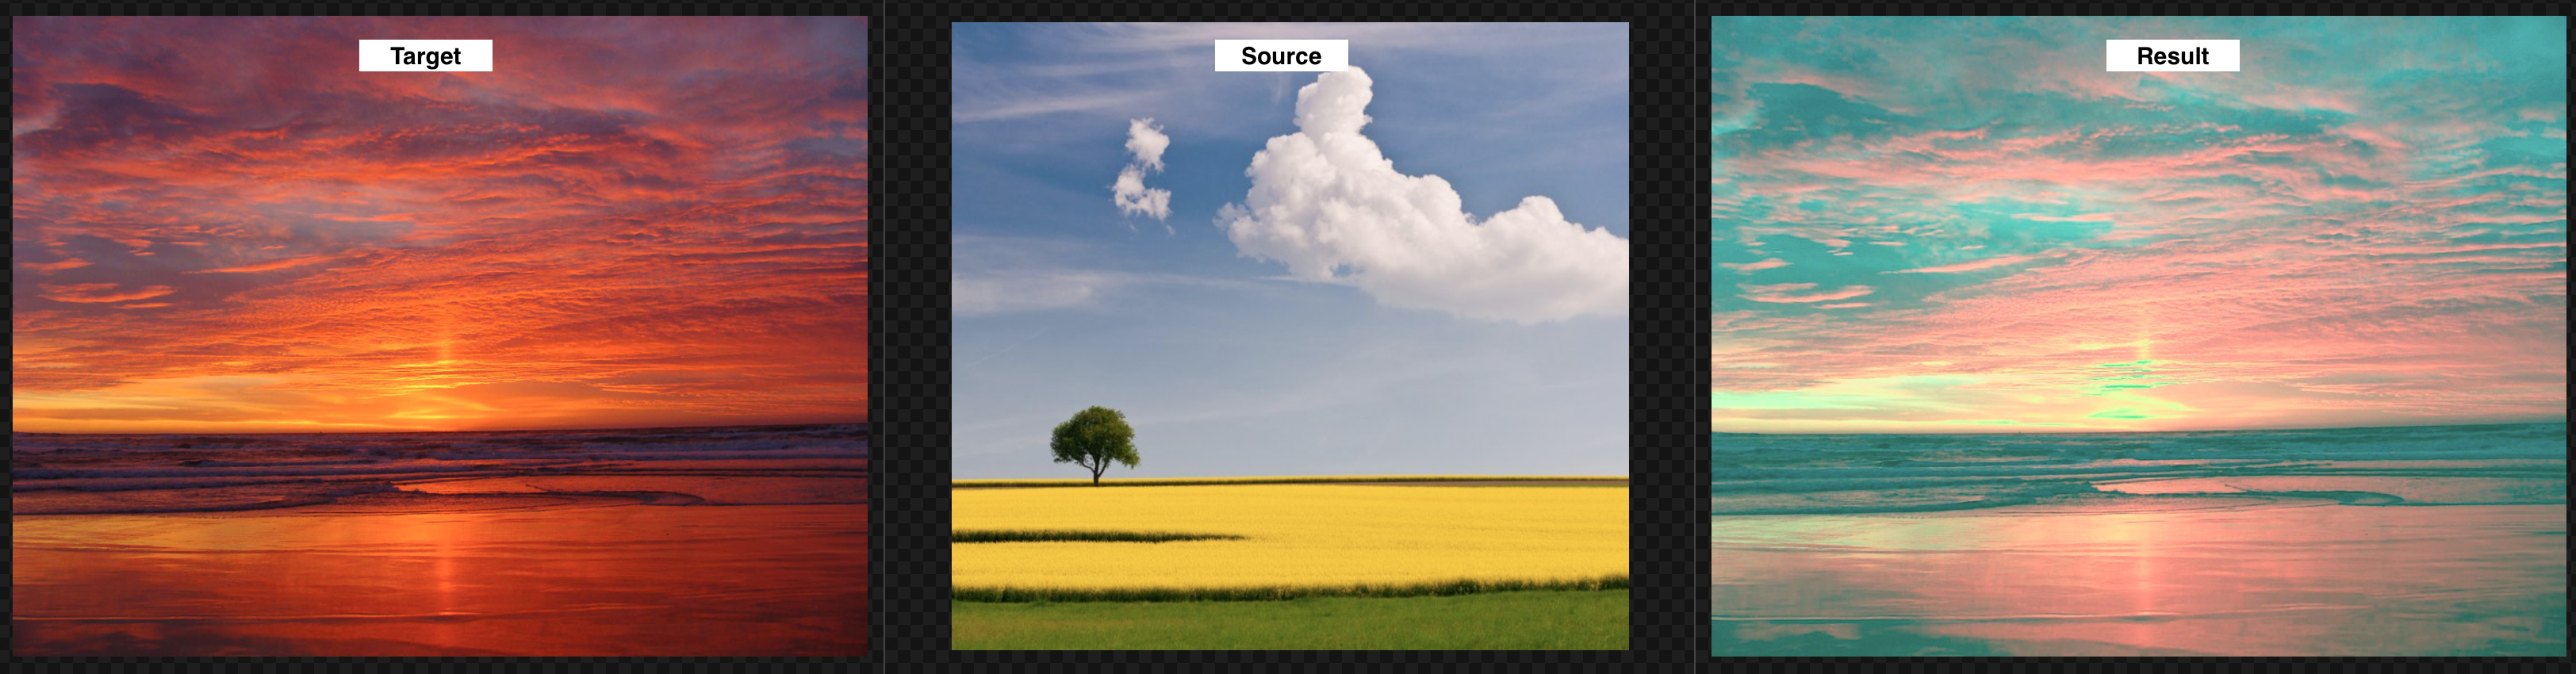
\includegraphics[width=\columnwidth]{6-Implementation/figs/color-transfer-exp-2.png}
            \caption{Color transfer - example 2}
        \end{figure}

        \begin{figure}[!h]\centering
            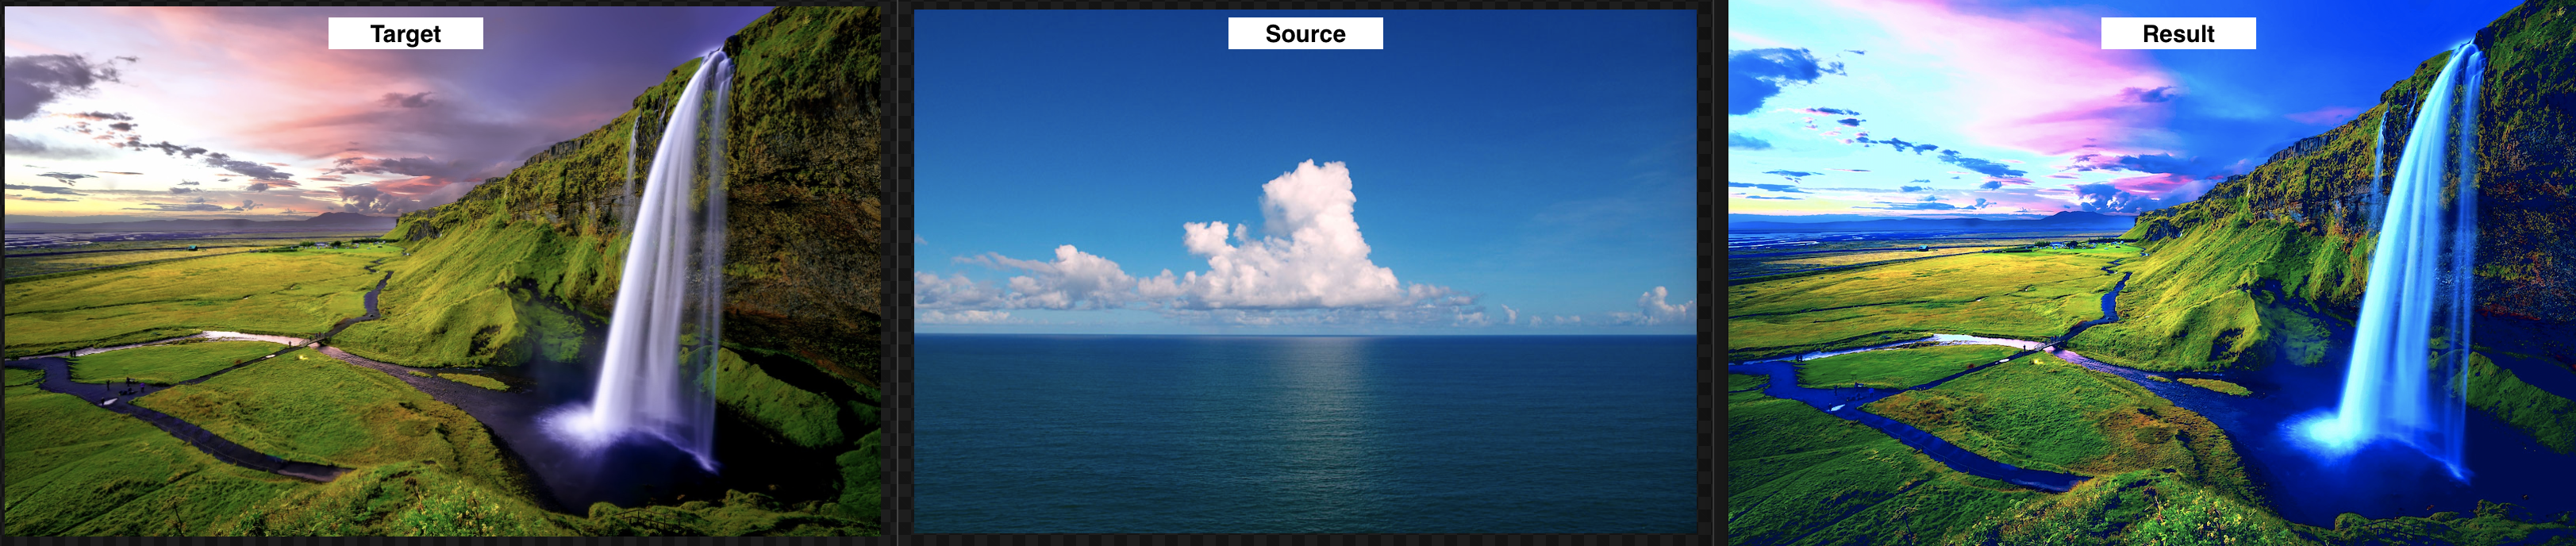
\includegraphics[width=\columnwidth]{6-Implementation/figs/color-transfer-exp-3.png}
            \caption{Color transfer - example 3}
        \end{figure}


        Github repository\cite{color-transfer}

    \end{itemize}


    \subsection{Documentation}
        Documentation is an extremely important part of any kind of project. To keep track of all informations
        concerning the project we used Attlassian Confluence which is a collaboration software
        program developed and published by Australian software company Attlassian to help teams collaborate
        and share knowledge efficiently. With Confluence, users can create pages and blogs which can be
        commented on and edited by all members of the team.

%******************************** Section 5.5 *********************************%
\section{Illustration}
    In this last section, we illustrate the project with pictures of the worker, the solar panel, the battery
    and the sensors and all the components together. At the end, we show a completed execution example.

    \begin{figure}[!h]\centering
        \includegraphics[width=\columnwidth]{6-Implementation/figs/illustration-1.jpg}
        \caption{The solar panel}
    \end{figure}

    \begin{figure}[!h]\centering
        \includegraphics[width=\columnwidth]{6-Implementation/figs/illustration-2.jpg}
        \caption{The Raspberry Pi worker}
    \end{figure}

    \begin{figure}[!h]\centering
        \includegraphics[width=\columnwidth]{6-Implementation/figs/illustration-3.jpg}
        \caption{The battery}
    \end{figure}

    \begin{figure}[!h]\centering
        \includegraphics[width=\columnwidth]{6-Implementation/figs/illustration-4.jpg}
        \caption{The global system}
    \end{figure}

    \begin{figure}[!h]\centering
        \includegraphics[width=\columnwidth]{6-Implementation/figs/illustration-5.jpg}
        \caption{The surveillance camera}
    \end{figure}

    \begin{figure}[!h]\centering
        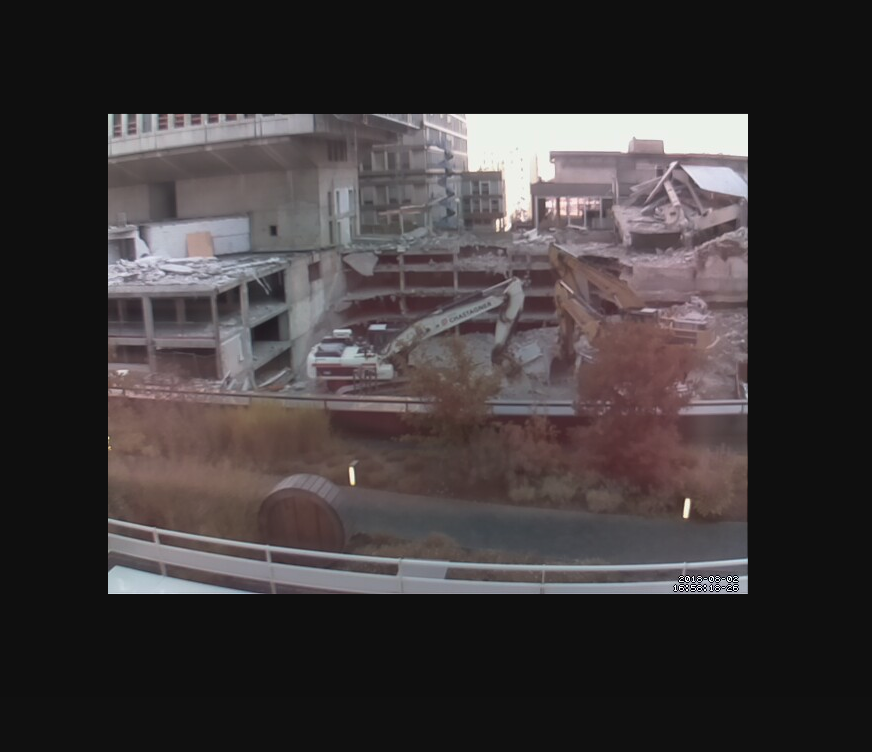
\includegraphics[width=\columnwidth]{6-Implementation/figs/illustration-8.png}
        \caption{Streamed video from the camera}
    \end{figure}

    \begin{figure}[!h]\centering
        \includegraphics[width=\columnwidth]{6-Implementation/figs/illustration-6.jpg}
        \caption{The weather station}
    \end{figure}

    \begin{figure}[!h]\centering
        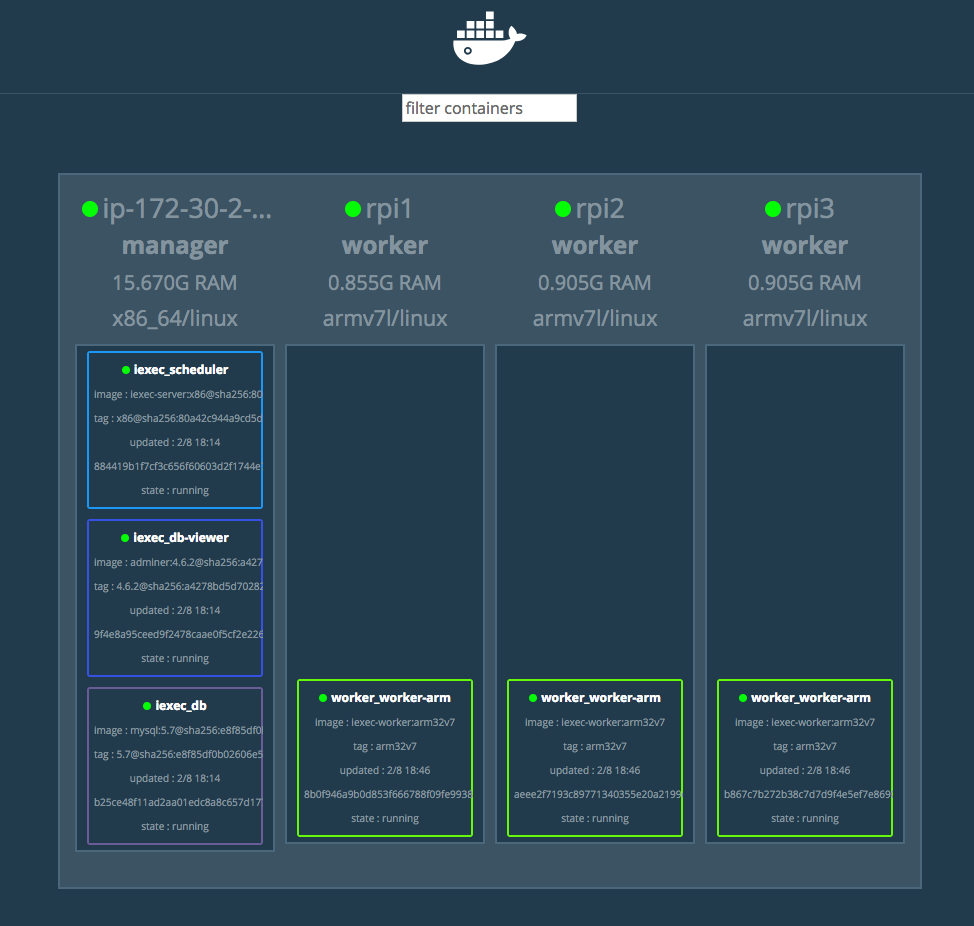
\includegraphics[width=\columnwidth]{6-Implementation/figs/illustration-7.png}
        \caption{The cluster of Raspberry Pi workers}
    \end{figure}

    \begin{figure}[!h]\centering
        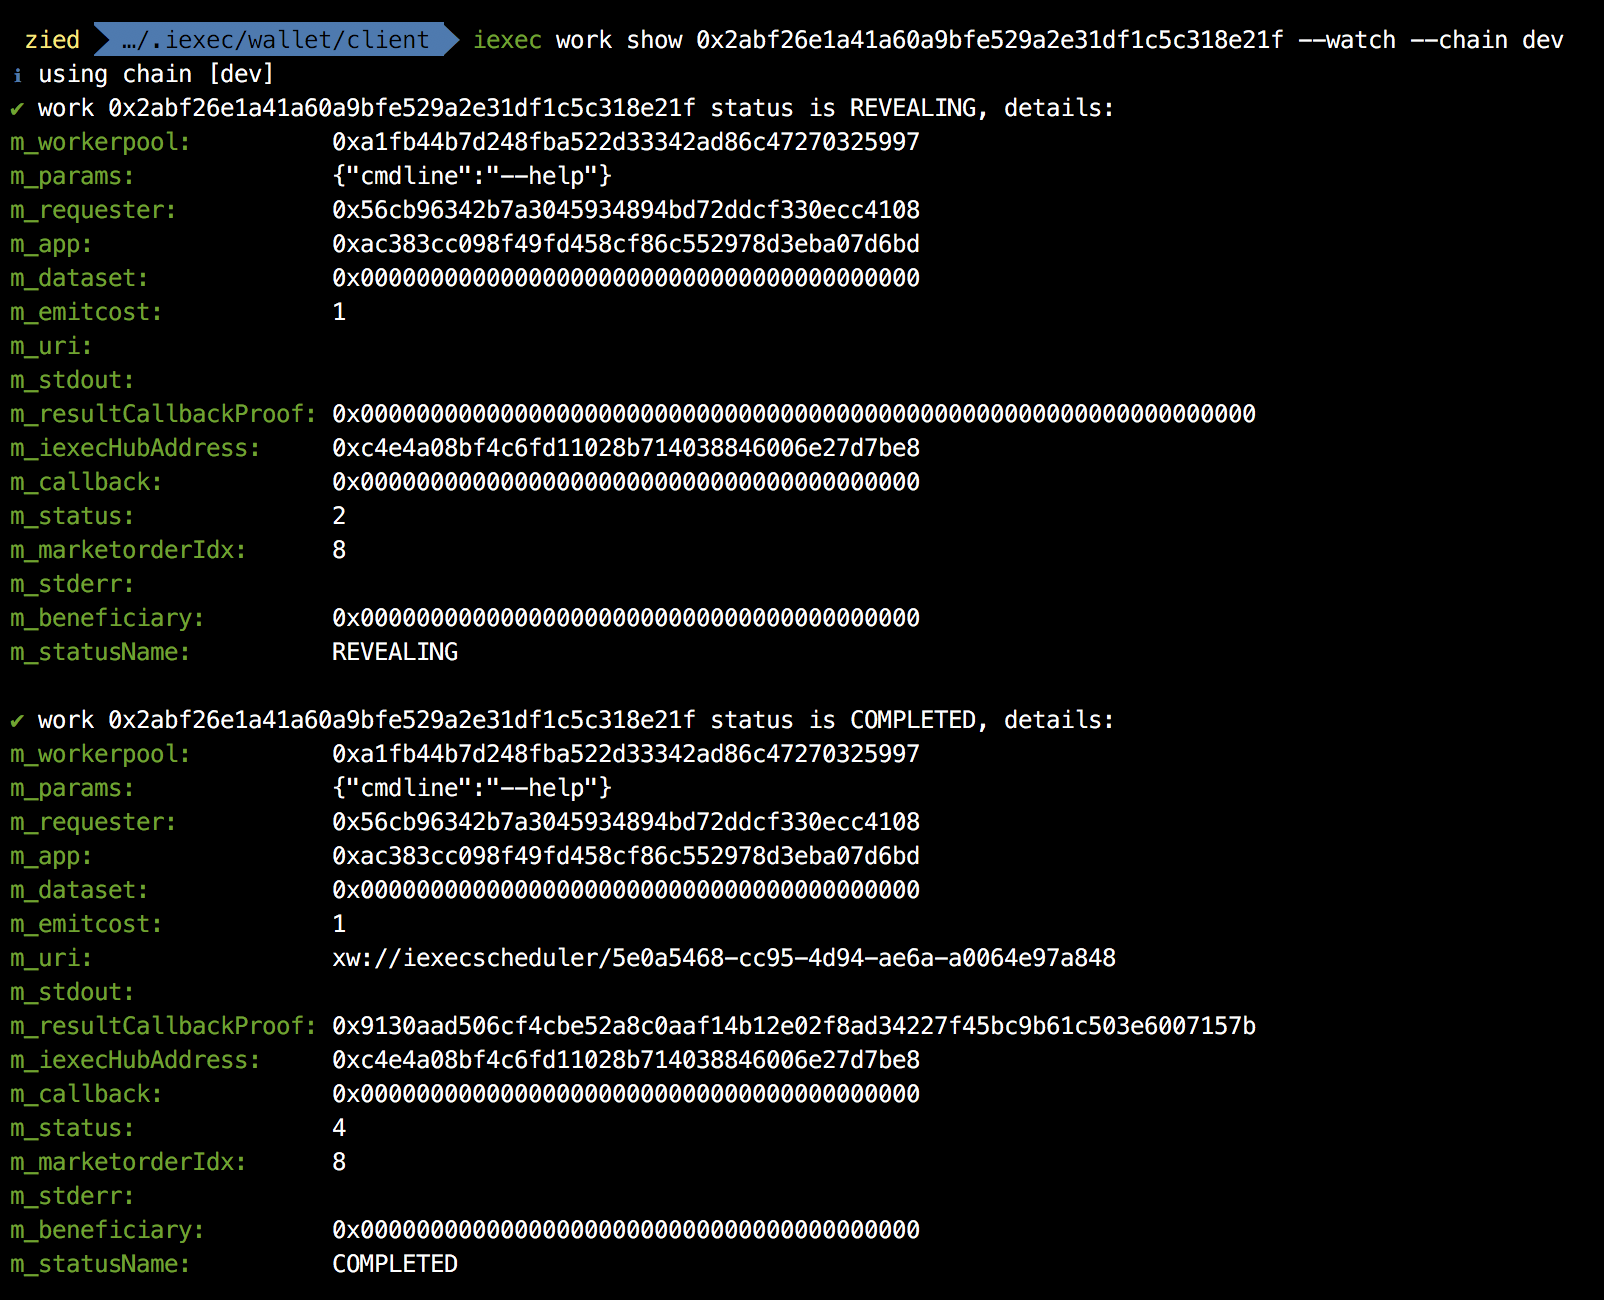
\includegraphics[width=\columnwidth]{6-Implementation/figs/illustration-9.png}
        \caption{Completed execution with job's informations}
    \end{figure}

    \clearpage

%******************************** Section 5.6 *********************************%
\section{Conclusion}
    Throughout this chapter, we have presented the details of the implementation of our system by demonstrating
    how we satisfied our requirements and showing some statistics and illustrative pictures.
    Finally, this section allowed us to crown the previous phases.